\documentclass[10pt, landscape]{article}
\usepackage[scaled=0.92]{helvet}
\usepackage{calc}
\usepackage{multicol}
\usepackage[a4paper,margin=3mm,landscape]{geometry}
\usepackage{amsmath,amsthm,amsfonts,amssymb}
\usepackage{color,graphicx,overpic}
\usepackage{hyperref}
\usepackage{newtxtext} 
\usepackage{enumitem}
\usepackage[table]{xcolor}
\usepackage{mathtools}
\setlist{nosep}
% for including images
\graphicspath{ {./images/} }

\pdfinfo{
  /Title (CS3236.pdf)
  /Creator (TeX)
  /Producer (pdfTeX 1.40.0)
  /Author (Jovyn Tan)
  /Subject (CS3236)
/Keywords (CS3236, nus,cheatsheet,pdf)}

% Turn off header and footer
\pagestyle{empty}

% redefine section commands to use less space
\makeatletter
\renewcommand{\section}{\@startsection{section}{1}{0mm}%
  {-1ex plus -.5ex minus -.2ex}%
  {0.5ex plus .2ex}%x
{\normalfont\large\bfseries}}
\renewcommand{\subsection}{\@startsection{subsection}{2}{0mm}%
  {-1explus -.5ex minus -.2ex}%
  {0.5ex plus .2ex}%
{\normalfont\normalsize\bfseries}}
\renewcommand{\subsubsection}{\@startsection{subsubsection}{3}{0mm}%
  {-1ex plus -.5ex minus -.2ex}%
  {1ex plus .2ex}%
{\normalfont\small\bfseries}}%
\makeatother

\renewcommand{\familydefault}{\sfdefault}
\renewcommand\rmdefault{\sfdefault}
%  makes nested numbering (e.g. 1.1.1, 1.1.2, etc)
\renewcommand{\labelenumii}{\theenumii}
\renewcommand{\theenumii}{\theenumi.\arabic{enumii}.}
\renewcommand\labelitemii{•}
\renewcommand\labelitemiii{•}

\definecolor{mathblue}{cmyk}{1,.72,0,.38}
\everymath\expandafter{\the\everymath \color{mathblue}}

% Don't print section numbers
\setcounter{secnumdepth}{0}

\setlength{\parindent}{0pt}
\setlength{\parskip}{0pt plus 0.5ex}
%% adjust spacing for all itemize/enumerate
\setlength{\leftmargini}{0.5cm}
\setlength{\leftmarginii}{0.5cm}
\setlist[itemize,1]{leftmargin=2mm,labelindent=1mm,labelsep=1mm}
\setlist[itemize,2]{leftmargin=4mm,labelindent=1mm,labelsep=1mm}

% adding my commands
% tightcenter
\newenvironment{tightcenter}{%
  \setlength\topsep{0pt}
  \setlength\parskip{0pt}
  \begin{center}
    }{%
  \end{center}
}

% boxed
\newenvironment{tightbox}{%
  \setlength\topsep{0pt}
  \setlength\parskip{0pt}
  \begin{center}
    \begin{tabular}{|@{\hspace{\dimexpr\fboxsep+0.5\arrayrulewidth}}c@{\hspace{\dimexpr\fboxsep+0.5\arrayrulewidth}}|}
      \hline
    }
    {%
    \\ \hline
    \end{tabular}
  \end{center}
}

% fixed width box
\newenvironment{fixedbox}[1][0.7]{
  \setlength\topsep{0pt}
  \setlength\parskip{0pt}
  \begin{center}
    \begin{tabular}{|>{\centering\arraybackslash}m{#1\linewidth}|}
    \hline
  }{
  \\ \hline
  \end{tabular}
  \end{center}
}

% definition of a new term
\usepackage{soul}
\definecolor{paleyellow}{RGB}{251,243,218}
\newcommand{\definition}[2][]{\sethlcolor{paleyellow}\hl{\textbf{#2}} #1  $\rightarrow$}

% important note (attention)
\newcommand{\attention}{{\color{red}\textbf{! }}}



% -----------------------------------------------------------------------

\begin{document}
\raggedright
\footnotesize
\begin{multicols*}{4}
  % multicol parameters
  \setlength{\columnseprule}{0.25pt}

  \begin{center}
    \fbox{%
      \parbox{0.8\linewidth}{\centering \textcolor{black}{
          {\Large\textbf{CS3236}}
        \\ \normalsize{AY22/23 SEM 2}}
        \\ {\footnotesize \textcolor{gray}{github/jovyntls}}
      }%
    }
  \end{center}

  \section{00. INTRODUCTION}

  \subsection{data compression}

  \begin{itemize}
    \item types of compression
      \begin{itemize}
        \item \textbf{lossless compression} - can recover the contents
        \item \textbf{lossy compression} - lose some quality - cannot convert back to the higher-quality version
      \end{itemize}
    \item examples
      \begin{itemize}
        \item sparse binary string - storing positions of 1s
        \item equal number of 0/1s - $L \geq \log_2 \binom{64}{32} \approx 60.7$
        \item english text - using relative frequency
        \item morse code is NOT binary (contains spaces)
      \end{itemize}
    \item info theory uses \textbf{probabilistic models} (letter frequency, sequence probabilities)
    \item 2 distinct approaches to compression:
      \begin{itemize}
        \item \textbf{variable length} - map more probable sequences to shorter binary strings
        \item \textbf{fixed length} - map most probable sequences to strings of a given length
          \begin{itemize}
            \item insufficient strings for low-probability sequences 
            \item tradeoff between length/failure probability
          \end{itemize}
      \end{itemize}
  \end{itemize}

  \subsection{information theory concepts}
  \begin{itemize}
    \item speed: \definition{rate} $\frac{k}{n}$ (mapping $k$ bits to $n$ bits)
    \item reliability: $ \mathbb{P}[error] $ = $\mathbb{P}[\text{estimated msg $\neq$ true msg}]$
    \item \definition{source coding theorem} the fundamental compression limit is given by a source-dependent quantity known as the \textbf{(Shannon) entropy $H$}. The (average) storage length can be arbitrarily close to $H$, but can never be any lower than $H$.
      \begin{itemize}
        \item $H$ is a property of the \textit{probability distribution}
      \end{itemize}
    \item \definition{channel coding theorem} there exists a channel-dependent quantity called the \textbf{(Shannon) capacity $C$} such that arbitrarily small error probability can be achieved only for rates $<C$
      \begin{itemize}
        \item can achieve $ \mathbb{P}[error] \leq \epsilon \iff$ rate $<C$
      \end{itemize}
  \end{itemize}

  \subsection{data communication example}

  \begin{itemize}
    \item a "transmitter" sends a sequence of 0s and 1s
    \item a "receiver" sends a sequence \textit{with some corruptions}
  \end{itemize}

  \subsubsection{channel transition diagram}

  \begin{minipage}[c]{0.3\linewidth}
    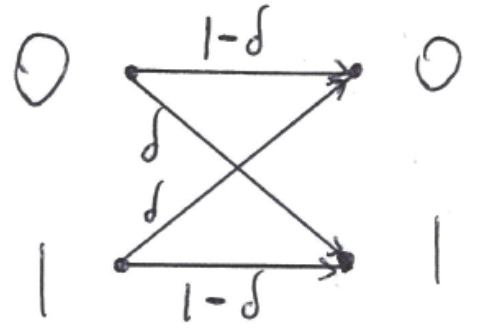
\includegraphics[width=0.8\linewidth]{cs3236-channel-transition-diagram.png} 
  \end{minipage}
  \begin{minipage}[c]{0.65\linewidth}
    \begin{itemize}
      \item each bit is flipped independently with probability $\delta \in (0, \frac{1}{2})$
    \end{itemize}
  \end{minipage}

  \subsubsection{naive}

  \begin{itemize}
    \item \textbf{uncoded communication} - $\mathbb{P}[correct] = (1-\delta)^N $
    \item \textbf{repetition code} - transmit "000" for "0", "111" for "1"
      \begin{itemize}
        \item $ \mathbb{P}[correct] = [(1-\delta)^3 + 3\delta(1-\delta)^2]^N $
        \item more reliable but 3x slower!
      \end{itemize}
  \end{itemize}

  \subsubsection{Hamming code}

  \begin{itemize}
    \item able to correct one bit flip
    \item maps binary string of length 4 to binary string of length 7
    \item fill in $b_1b_2b_3b_4$ and assign $c_1c_2c_3$ such that the sum of bits in each circle is even
      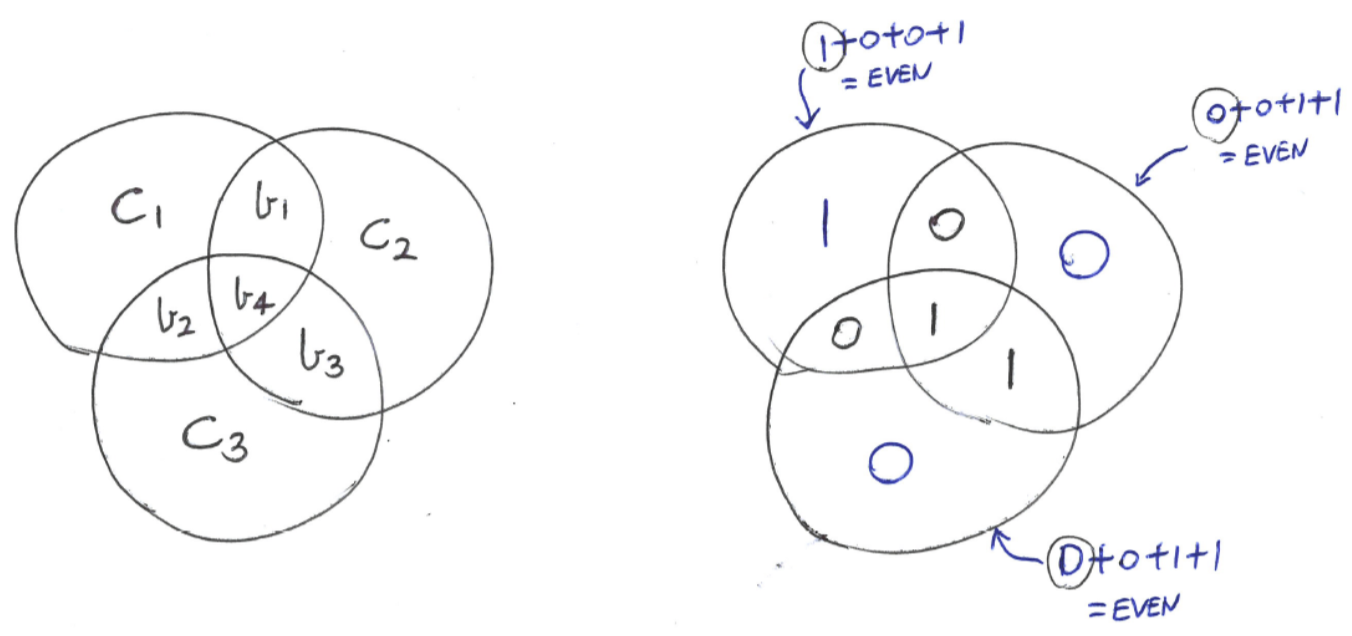
\includegraphics[width=0.8\linewidth]{cs3236-hamming-example.png} 
    \item $ \mathbb{P}[correct] \geq \mathbb{P}[\leq 1\text{bit flips}] = (1-\delta)^7 + 7\delta(1-\delta)^6 $
    \item with $\delta=1$: Shannon capacity $C\approx 0.531$ 
  \end{itemize}

  \section{01. INFORMATION MEASURES}

  \subsection{information of an event}

  \begin{itemize}
    \item \definition{entropy} measure of "uncertainty" or "information" in a random variable
    \item given event $A$ with some $\mathbb{P}[A] = p$, how much "information" learned by being told $A$ occurred?
      \begin{itemize}
        \item only $ \mathbb{P}[A] $ matters
      \end{itemize}
    \item if $A$ occurs with probability $p$, then $\quad Information(A) = \psi(p)$ for some function $\psi(\cdot)$
  \end{itemize}

  \subsubsection{axioms for $\psi(\cdot)$}

  \begin{tightcenter}
    \( {\displaystyle{ \psi(p) = \log_b \frac{1}{p} }} \) (for some base $b>0$)
  \end{tightcenter}

  we gain $\log_2 \frac{1}{p}$ "bits" of info if a probability-$p$ event occurs.

  \begin{minipage}[c]{0.3\linewidth}
    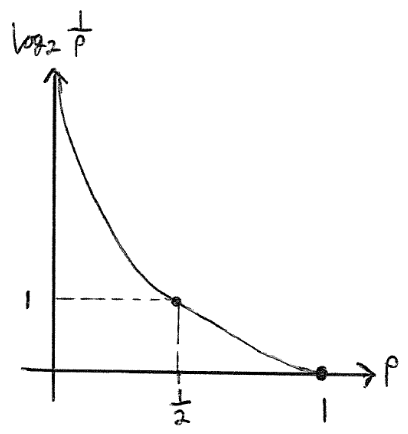
\includegraphics[width=0.95\linewidth]{cs3236-information-log2-p-graph.png} 
  \end{minipage}
  \begin{minipage}[c]{0.67\linewidth}
    \begin{itemize}
      \item only $\psi(p) = \log_b\frac{1}{p}$  satisfies all axioms
      \item we focus on $b=2$ 
        \begin{itemize}
          \item information measured in bits
        \end{itemize}
      \item all choices of $b$ are equivalent up to scaling by a universal constant
        \begin{itemize}
          \item e.g. \# of nats $= \log_e 2 \times$ \# of bits
        \end{itemize}
    \end{itemize}
  \end{minipage}

  \begin{enumerate}
    \item $\psi(p) \geq 0\quad$ (\textbf{non-negativity}) 
    \item $\psi(1) = 0\quad$ (\textbf{zero for definite events}) 
    \item if $p \leq p'$, then $\psi(p) \geq \psi(p') \quad$ (\textbf{monotonicity})
      \begin{itemize}
        \item the less likely an event is, the more information was learnt by the fact that it occurred
      \end{itemize}
    \item $\psi(p)$ in continuous in $p \quad$ (\textbf{continuity}) 
      \begin{itemize}
        \item small change in probability: no drastic change in info
      \end{itemize}
    \item $\psi(p_1 p_2) = \psi(p_1) + \psi(p_2)\quad$  
      \begin{itemize}
        \item (\textbf{additivity under independence}) if $A$ and $B$ are independent events with probabilities $p_1$ and $p_2$, then $\mathbb{P}[A \cap B]=p_1p_2$, and the information learnt from both $A$ and $B$ occurring is the sum of the two individual amounts of information (because they are independent)
        \item $\psi(\mathbb{P}[A_1 \cap A_2]) = \psi(\mathbb{P}[A_1]) + \psi(\mathbb{P}[A_2])$
      \end{itemize}
  \end{enumerate}


  \subsection{information of a random variable - entropy}

  \begin{itemize}
    \item let $X$ be a discrete r.v. with pmf $P_X$
    \item if we observe $X=x$ then we have learnt $\log_2 \frac{1}{P_X(x)}$ bits of information
  \end{itemize}

  \begin{tightcenter}
    \textbf{(Shannon) entropy} \\* is the average \textit{information/uncertainty} in $X$ wrt $P_X$:
    \begin{align*}
      H(X) &= \mathbb{E }_{X \sim P_X} \left[ \log_2 \frac{1}{P_X(X)} \right] 
        \\ &= \sum_x P_X(x) \log_2 \frac{1}{P_X(x)}
    \end{align*}
  \end{tightcenter}

  \begin{itemize}
    \item \definition{binary entropy function} \( {\displaystyle{ \quad\quad H_2(p) = p\log_2 \frac{1}{p} + (1-p) \log_2 \frac{1}{1-p} }} \) 
    \item e.g. 
      \begin{itemize}
        \item binary source: $X \sim Bernoulli(p)$, $\quad p \in (0,1)$ \\* $\quad \Rightarrow H(X) = H_2(p)$
        \item uniform source: $X$ is uniform on a finite set $\mathcal{X}$ 
          \begin{itemize}
            \item $P_X(x) = \frac{1}{\vert \mathcal{X} \vert}$
          \end{itemize}
          $\quad \Rightarrow$ $H(X) = \mathbb{E} \left[ \log_2 \frac{1}{1/\vert\mathcal{X}\vert} \right] = \log_2 \vert\mathcal{X}\vert$
      \end{itemize}
    \item entropy $\neq$ variance
      \begin{itemize}
        \item entropy depends \textit{only} on the probability values
      \end{itemize}
  \end{itemize}

  \subsubsection{axiomatic view (Shannon)}

  $X$ is a d.r.v. taking $N$ values with $\mathbf{p} = (p_1, \dots, p_N)$. We consider a general information measure of the form 
  \centerline{$\Phi(\mathbf{p}) = \Phi (p_1, \dots, p_N)$}

  \begin{tightcenter}
    only  $\Phi(X) = constant \times H(X)$ satisfies all axioms.
  \end{tightcenter}

  \begin{enumerate}
    \item $\Psi(\mathbf{p})$ is continuous on $p \quad$ (\textbf{continuity}) 
    \item if $p_i= \frac{1}{N}$, then $\Psi(\mathbf{p}) $ is increasing in $N$ (\textbf{uniform case})
      \begin{itemize}
        \item uniformity over a larger set of outcomes always means more uncertainty
      \end{itemize}
    \item (\textbf{successive decisions}) $\Psi(p_1, \dots, p_N) = \Psi(p_1 + p_2, p_3, \dots, p_N) + (p_1 + p_2) \Psi (\frac{p_1}{p_1 + p_2}, \frac{p_2}{p_1 + p_2})$
  \end{enumerate}

  \subsubsection{variations}

  \begin{itemize}
    \item \definition[ of two random variables $(X, Y)$ ]{joint entropy}
      \begin{align*}
        H(X,Y) &= \mathbb{E}_{(X, Y)\sim P_{XY}} \left[ \log_2 \frac{1}{P_{XY}(X,Y)} \right] 
            \\ &= \sum_{x,y} P_{XY} (x,y) \log_2 \frac{1}{P_{XY}(x,y)}
      \end{align*}
    \item \definition[ of $Y$ given $X$ ]{conditional entropy}
      \begin{align*}
        H(Y\vert X) &= \mathbb{E}_{(X,Y) \sim P_{XY}} \left[ \log_2 \frac{1}{P_{Y\vert X}(Y\vert X)} \right] 
                 \\ &= \sum_{x, y} P_{XY}(x,y) \log_2  \frac{1}{P_{Y\vert X}(y\vert x)}
                 \\ &= \sum_x P_X(x) H(Y \vert X=x)
      \end{align*}
      \begin{itemize}
        \item on average, knowing $X$ reduces uncertainty about $Y$ ($H(Y\vert X) \leq H(Y)$), but seeing a \textit{specific} outcome of $X$ may increase uncertainty about $Y$ ($H(Y \vert X=i) > H(Y)$ for some values of $i$)
      \end{itemize}
  \end{itemize}

  \subsection{properties of entropy}

  \begin{enumerate}
    \item $H(X) \geq 0 \quad$ (\textbf{non-negativity})
      \begin{itemize}
        \item $H(X)=0 \iff X$ if deterministic
        \item \textit{Proof.} information $\log_2\frac{1}{p} \geq 0$ for $p \in [0,1]$, so entropy is the average of a non-negative quantity, and itself is non-negative
      \end{itemize}
    \item $H(X) \leq \log_2 \vert\mathcal{X}\vert \quad$ (\textbf{upper bound}) \\* if $X$ takes values on a finite alphabet $ \mathcal{X} $
      \begin{itemize}
        \item $H(X) = \log_2\vert \mathcal{X}\vert \iff X\sim Uniform(\mathcal{X})$
        \item implies $\quad H(X \vert Y) \leq \log_2 \vert \mathcal{X} \vert$
      \end{itemize}
    \item $H(X, Y) = H(X) + H(Y\vert X) \quad$ (\textbf{chain rule})
      \begin{itemize}
        \item or $H(X, Y) = H(Y) + H(X\vert Y)$
        \item overall information in $(X, Y)$ is the information in $X$ plus the remaining information in $Y$ after observing $X$.
        \item with conditioning: $H(X, Y \vert Z) = H(X \vert Z) + H(Y \vert X, Z)$
        \item general chain rule: $H(X_1, \dots, X_n) = \sum^n_{i=1} H(X_i \vert X_1, \dots, X_{i-1})$
      \end{itemize}
    \item $H(X \vert Y) \leq H(X) \quad$ (\textbf{conditioning reduces entropy})
      \begin{itemize}
        \item $H(X \vert Y) = H(X) \iff X$ and $Y$ are independent
        \item additional information $Y$ can't increase uncertainty \textit{on average}
          but \textit{can} have $H(X \vert Y=y) > H(X)$
      \end{itemize}
    \item $H(X_1, \dots, X_n) \leq \sum^n_{i=1} H(X_i) \quad$ (\textbf{sub-additivity})
      \begin{itemize}
        \item equality $\iff X$ and $Y$ are independent
      \end{itemize}
  \end{enumerate}

  \subsection{KL Divergence}

  \begin{tightcenter}
    for two pmfs $P$ and $Q$ on a finite alphabet $\mathcal{X}$, the \ildefinition{Kullback-Leibler (KL) divergence} or \ildefinition{relative entropy} is given by
    \begin{align*}
      D(P||Q) &= \sum_x P(x) \log_2 \frac{P(x)}{Q(x)} \\*
              &= \mathbb{E}_{X \sim P}  \left[ \log_2 \frac{P(X)}{Q(X)} \right]
    \end{align*}
  \end{tightcenter}

  \begin{itemize}
    \item $D(P||Q) \neq D(Q||P)$
    \item $D(P||Q) \geq 0 \quad$ 
      \begin{itemize}
        \item \textit{Proof.} $-D(P||Q) = - \sum_x P(x) \log_2 \frac{P(x)}{Q(x)}$  
          $\leq \sum_x P(x) (\frac{Q(x)}{P(x)}-1) = \sum_x Q(x) - \sum_x P(x) = 0$ 
          \\* (using property that $\log \alpha \leq \alpha-1$, equality iff $\alpha=1$)
      \end{itemize}
    \item $D(P||Q) = 0 \iff P=Q$
      \begin{itemize}
        \item \textit{Proof.} same as above, with $\ln \alpha = \alpha-1 \iff \alpha=1$ (then $\frac{P(x)}{Q(x)} = 1$)
      \end{itemize}
  \end{itemize}

  \subsection{Mutual Information}

  \begin{align*}
    I(X;Y) &= H(Y) - H(Y \vert X) \\*
           &= H(X) - H(X \vert Y) \\*
           &= H(X) + H(Y) - H(X, Y) \\*
           &= D(P_{XY}\vert\vert P_X \times P_Y)
  \end{align*}

  \begin{itemize}

    \item \definition[, $I(X;Y)$]{mutual information} the amount of information we learn about $Y$ by observing $X$ (on avg)
      \begin{itemize}
        \item $H(Y)$ = uncertainty in  $Y$ 
        \item $H(Y \vert X)$ = (avg) uncertainty in $Y$ after observing $X$
        \item $D(P_{XY}\vert\vert P_X P_Y)$ = how far $X,Y$ are from being independent
      \end{itemize}
    \item $I(X_1;X_2,X_3) \neq I(X_1, X_2;X_3)$ 
    \item \definition{joint mutual information} 
      \begin{align*}
        I(X_1, X_2 ; Y_1, Y_2) = H(Y_1, Y_2) - H(Y_1, Y_2 \vert X_1, X_2)
      \end{align*}
    \item \definition{conditional mutual information} 
      \begin{align*}
        I(X;Y \vert Z) = H(Y \vert Z) - H(Y \vert X,Z)
      \end{align*}
    \item if $X \perp Y$, then $I(X;Y) = 0$ 
      \begin{itemize}
        \item \textit{Proof}. $X \perp Y \Rightarrow P_{XY} = P_X \times P_Y \Rightarrow D(P_{XY} \vert \vert P_X \times P_Y) = 0$
        \item independent variables do not reveal any information about each other
      \end{itemize}
    \item if  $X=Y$, then $I(X;Y) = H(X) = H(Y)$
      \begin{itemize}
        \item amt of information a r.v. reveals about itself is the entropy
      \end{itemize}
  \end{itemize}

  \subsubsection{properties of mutual information}

  \begin{enumerate}
    \item $I(X; Y) = I(Y;X) \quad$ (\textbf{symmetry})
      \begin{itemize}
        \item $X$ and $Y$ reveal an equal amount of information about each other
      \end{itemize}
    \item $I(X;Y) \geq 0 \quad $ (\textbf{non-negativity})
      \begin{itemize}
        \item equality $\iff X \perp Y$
      \end{itemize}
    \item $I(X;Y) \leq H(X) \leq \log_2 \vert \mathcal{X} \vert \quad$ (\textbf{upper bounds}) 
      \\* $I(X;Y) \leq H(Y) \leq \log_2 \vert \mathcal{Y} \vert$
      \begin{itemize}
        \item the information $X$ reveals about $Y$ is \textit{at most} the prior information in $X$ (entropy)
      \end{itemize}
    \item  $I(X,Y;Z) = I(X;Z) + I(Y;Z\vert X)$ $\quad$ (\textbf{chain rule})
      \\* \( {\displaystyle{ I(X_1, \dots, X_n;Y) = \sum^n_{i=1} I(X_i; Y \vert X_1, \dots, X_{i-1}) }} \) 
      \\* $ \quad\quad\quad\quad\quad\quad\quad\quad = I(X_1;Y) + I(X_2;Y \vert X_1) + \dots$
    \item (\textbf{data-processing inequality})
      \\* $I(X;Z) \leq I(X;Y)$ if $X \rightarrow Y \rightarrow Z$
      \\* $\quad$ variation: $I(X;Z) \leq I(Y;Z)$ if $X \rightarrow Y \rightarrow Z$
      \\* $I(W;Z) \leq I(X;Y)$ if $W \rightarrow X \rightarrow Y \rightarrow Z$ $\quad$  
      \begin{itemize}
        \item holds if $Z$ depends on $(X, Y)$ only through $Y$ (i.e. $X \rightarrow Y \rightarrow Z$ forms a \textbf{Markov chain})
        \item processing $Y$ (to produce $Z$)  cannot increase the information available regarding $X$
          \begin{itemize}
            \item cannot do data processing to increase information
          \end{itemize}
      \end{itemize}
    \item (\textbf{partial sub-additivity}) 
      \\*  \( {\displaystyle{ I(X_1, \dots, X_n; Y_1, \dots, Y_n) \leq \sum^n_{i=1} I(X_i;Y_i) }} \) 
      \\* if $(Y_1, \dots, Y_n)$ are conditionally independent given $(X_1, \dots, X_n)$, and $Y_i$ depends on $(X_1, \dots, X_n)$ only through $X_i$
  \end{enumerate}


  \section{02. SYMBOL-WISE SOURCE CODING}

  $X$ is a d.r.v. with pmf $P_X$ over an alphabet $\mathcal{X}$ (set of symbols).

  \begin{tightcenter}
    \ildefinition{symbol-wise source coding} maps each $x \in \mathcal{X}$ to some binary sequence $C(x)$ of length  $\ell(x)$.
  \end{tightcenter}
  \begin{tightcenter}
    \textbf{average length} of a code $C(\cdot)$, 
    \\* \( {\displaystyle{ L(C) = \sum_{x \in \mathcal{X}} P_X(x) \ell (x) }} \) 
  \end{tightcenter}

  \subsubsection{decodability conditions}
  \begin{itemize}
    \item \definition{nonsingular property} $C(x) \neq C(x') \iff x\neq x'$
    \item $C(\cdot)$ is \definition{uniquely decodable} no 2 sequences (of equal or differing lengths) of symbols in $\mathcal{X}$ are coded to the same concatenated binary sequence.
      \begin{itemize}
        \item $x_1, \dots, x_n$ can be always uniquely identified from the string  $C(x_1) \dots C(x_n)$
      \end{itemize}
    \item $C(\cdot)$ is \definition{prefix-free} no codeword is a prefix of another
      \begin{itemize}
        \item aka \textbf{instantaneous code}
      \end{itemize}
  \end{itemize}

  \subsection{Kraft's Inequality and Entropy Bound}

  \begin{tightcenter}
    \ildefinition{Kraft's inequality} 
    \\* $\quad\quad$ if $C(\cdot)$ is \textit{prefix-free}, then \( {\displaystyle{\quad \sum_{x \in \mathcal{X}} 2^{-\ell(x)} \leq 1 }} \) 
  \end{tightcenter}

  \begin{itemize}
    \item \textit{Proof.} represent the codewords by a binary tree. If there is a codeword at some point in the tree, there are no codewords further down the tree. probability of branching to a codeword $=2^{-\ell (x)}$ and sum of probabilities cannot exceed 1
    \item \definition{existence property} if a given set of integers $\{ \ell(x) \}_{x \in \mathcal{X}}$ satisfies $\sum_{x \in \mathcal{X}} 2^{-\ell(x)} \leq 1$, 
      then it is possible to construct a \textit{prefix-free} code that maps each $x \in \mathcal{X}$ to a codeword of length $\ell(x)$.
  \end{itemize}

  \subsubsection{entropy bound}

  \begin{tightcenter}
    \ildefinition{entropy bound} \\*
    expected length, $L(C) \geq H(X)$
    \\* with equality $\iff P_X(x) = 2^{-\ell(x)} \quad\; \forall x \in \mathcal{X}$
  \end{tightcenter}

  \begin{itemize}
    \item entropy gives a \textit{fundamental compression limit}
      \begin{itemize}
        \item average length is at least equal to entropy
        \item if all probabilities are negative powers of 2, we can match the entropy bound (optimal code)
      \end{itemize}
    \item \textit{Proof.} manipulate to get $L(C) - H(X) \geq D(P_X||Q) \geq 0$
  \end{itemize}


  \subsection{Shannon-Fano Code}

  \begin{tightcenter}
    $\ell(x) = \left\lceil \log_2 \frac{1}{P_X(x)} \right\rceil $
  \end{tightcenter}

  \begin{itemize}
    \item \textbf{average length}, $L(C)$ satisfies
      \begin{tightcenter}
        $H(X) \leq L(C) < H(X) + 1$
      \end{tightcenter}
    \item \textbf{Kraft's inequality} holds - 
      \( {\displaystyle{ \sum_{x \in \mathcal{X}} 2^{-\ell (x)} 
      \leq \sum_{x \in \mathcal{X}} 2^{-\log_2 \frac{1}{P_X(x)} } = \sum_{x \in \mathcal{X}} P_X(x) = 1 }} \) 
      \begin{itemize}
        \item \textbf{Existence property} holds - we can construct a prefix-free code with these lengths 
      \end{itemize}
    \item 1 bit may be significant - e.g. if $H(X)=0.5$
    \item \textbf{mismatched case} - 
  \end{itemize}
  \begin{tightcenter}
    if the true distribution is $P_X$ but the lengths are chosen according to $Q_X$, 
    then the Shannon-Fano code satisfies
    $H(X) + D(P_X \vert \vert Q_X) \leq L(C) \leq H(X) + D(P_X \vert \vert Q_X) + 1$
  \end{tightcenter}


  \subsection{Huffman Code}

  \begin{itemize}
    \item no uniquely decodable symbol code can achieve a smaller length $L(C)$ than the Huffman code.
      \begin{itemize}
        \item always prefix-free
        \item satisfies average length bound (because it is at least as good as Shannon-Fano):
          $H(X) \leq L(C) < H(X) + 1$
      \end{itemize}
  \end{itemize}

  \begin{tightcenter}
    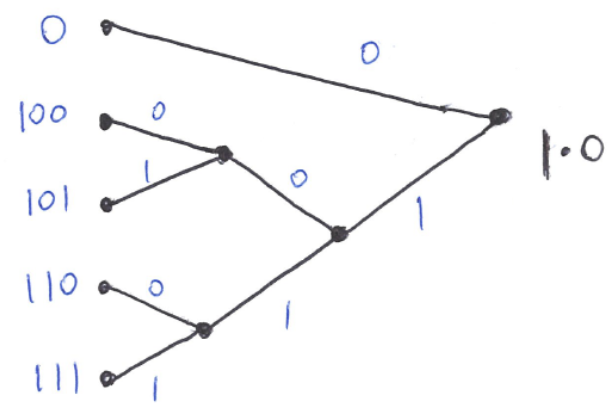
\includegraphics[width=0.6\linewidth]{cd3236-huffman-code-tree.png} 
  \end{tightcenter}

  \begin{itemize}
    \item extension: using blocks of $n$ letters; Huffman coding with $\mathcal{X}^n$ 
      \\* $nH(X) \leq L(C) < nH(X) + 1$
      \\* $\quad \Rightarrow H(X) \leq$ avg. length per symbol $\leq H(X) + \frac{1}{n}$
      \begin{itemize}
        \item $\checkmark$ exploits \textit{memory}, better guarantee (even independent)
        \item $\times$ but it's harder to accurately know $P_{X_1 \dots X_n}$
        \item $\times$  alphabet size increases to $\vert \mathcal{X} \vert^n$ $\Rightarrow$ expensive to sort
      \end{itemize}
  \end{itemize}

  \subsection{other codes}

  \begin{itemize}
    \item \textbf{arithmetic codes} - encodes a sequence $(x_1, \dots, x_n)$ to at most 
      $\ell(x_1, \dots, x_n) \leq \log_2 \frac{1}{P_{X_1, \dots, X_n} (x_1, \dots, x_n)} + 2$ 
      \begin{itemize}
        \item avg. length per letter $\leq H(X) + \frac{2}{n}$
      \end{itemize}
    \item \textbf{Lempel-Ziv code} - does not require knowledge of the source distribution 
      \begin{itemize}
        \item near-optimal: $O(\frac{\log n}{n})$ instead of $O(\frac{1}{n})$
      \end{itemize}
  \end{itemize}


  \section{03. BLOCK-WISE SOURCE CODING}

  \begin{itemize}
    \item aka \textbf{fixed-to-fixed} length source coding
    \item $\mathbb{P}[error] > 0$ (but small)
      \begin{itemize}
        \item map likely source strings, fail on unlikely source strings
      \end{itemize}
    \item instead of symbol-by-symbol, apply some encoding function to a length-$n$ block $X_1, \dots, X_n$
      \begin{itemize}
        \item map a string to some integer $m \in \{1, \dots, M\}$
      \end{itemize}
    \item \textbf{discrete memoryless source} $(X_1, \dots, X_n)$ 
      \begin{itemize}
        \item \textit{discrete} - the alphabet $\mathcal{X}$ is finite
        \item \textit{memoryless} - $P_{\underset{\sim}{X}}(\underset{\sim}{x}) = \Pi^n_{i=1} P_X(x_i)$
          \begin{itemize}
            \item every letter is independent (unrealistic)
          \end{itemize}
      \end{itemize}
      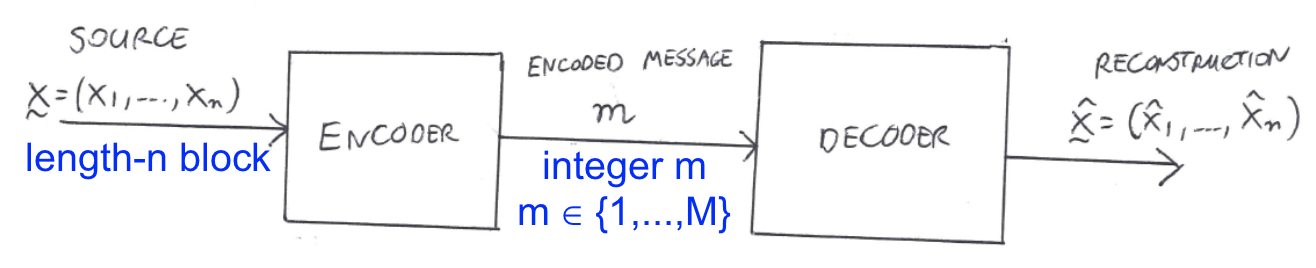
\includegraphics[width=0.9\linewidth]{cs3236-blockwise-source-coding.png} 
    \item \textit{decoder} maps $m$ to an estimate $\hat{\underset{\sim}{X}} = g(m)$  (in $\mathcal{X}^n$)
    \item \definition{error} occurs if $\hat{X} \neq X$
      \begin{itemize}
        \item $P_e = \mathbb{P}[\hat{\underset{\sim}{X}} \neq {\underset{\sim}{X}}] = \sum_{\underset{\sim}{x}: \textsc{DEC(ENC($x$))} \neq x} P_{\underset{\sim}{X}}(\underset{\sim}{x})$
      \end{itemize}
    \item \definition{rate} $R = \frac{1}{n}\log_2 M$
      \begin{itemize}
        \item ratio of compressed length ($\log_2 M$) to source length ($n$)
          \begin{itemize}
            \item represents the number of bits per source symbol used to represent encoded value $m$
          \end{itemize}
        \item number of strings we can compress to, $M = 2^{nR}$
        \item lower rate = more compression
        \item $R \leq H(X) + \epsilon$
          \begin{itemize}
            \item \textit{Proof}. $R = \frac{1}{n}\log_2 M = \frac{1}{n}\log_2 (|\mathcal{T}_n(\epsilon)| + 1)$ 
              \\* $\simeq \frac{1}{n} \log_2 |\mathcal{T}_n(\epsilon)| \leq H(X) + \epsilon$ (using property 3)
          \end{itemize}
      \end{itemize}
  \end{itemize}

  \begin{itemize}
    \item \definition{fixed length source coding theorem} for any discrete memoryless source with per-symbol distribution $P_X$, 
      \begin{itemize}
        \item (\textbf{achievability}) if $R>H(X)$, then for any $\epsilon > 0$, we can get $P_e \leq \epsilon$ for large enough $n$ 
        \item (\textbf{converse}) if $R<H(X)$, then there exists $\epsilon > 0$ such that $P_e > \epsilon$ for all $n$
      \end{itemize}
  \end{itemize}

  \subsection{Typical Sequences}

  for i.i.d. sequence $\mathbf{X} = (X_1, \dots, X_n)$, let $P_X(x) = \Pi^n_{i=1} P_X(x_i)$ be the pmf of $X$.

  \begin{center}
    \ildefinition{typical set}, \( {\displaystyle{ \mathcal{T}_n(\epsilon) = }} \) 
    \( {\displaystyle{ \left\{ x \in \mathcal{X}^n : 2^{-n(H(X) + \epsilon)} \leq P_X(x) \leq 2^{-n(H(X)-\epsilon)} \right\} }} \) 
    where $\epsilon > 0$ is a (small) fixed constant
    \\* i.e. $P_{\underset{\sim}{X}}({\underset{\sim}{x}}) \simeq 2^{-nH({\underset{\sim}{X}})}$
  \end{center}

  \begin{itemize}
    \item we only assign a (unique) $m \in \{1, \dots, M\}$ to \textit{some} ${\underset{\sim}{x}}$
      \begin{itemize}
        \item choose ${\underset{\sim}{x}}$ such that $\mathbb{P}[{\underset{\sim}{x}} \in \mathcal{T}_n(\epsilon)] \simeq 1$
      \end{itemize}
  \end{itemize}

  \subsubsection{properties of a typical set}

  for any fixed $\epsilon > 0$, 

  \begin{enumerate}
    \item (\textbf{equivalent definition}) $x \in \mathcal{T}_n(\epsilon) \iff$  
      \( {\displaystyle{ H(X) - \epsilon \leq \frac{1}{n} \sum^n_{i=1} \log_2 \frac{1}{P_X(x_i)} \leq H(X) + \epsilon }} \) 
      \\* where $x_i$ is the $i$-th entry of $x$
      \begin{itemize}
        \item $\mathbb{E}[\log P_X(x_i)] = H(X_i) = H(X)$
      \end{itemize}
    \item \( {\displaystyle{ \mathbb{P}[X \in \mathcal{T}_n(\epsilon)] \to 1 \;\; }} \)  as $n \to \infty \quad$ (\textbf{high probability})
    \item \( {\displaystyle{ \vert \mathcal{T}_n(\epsilon)\vert \leq 2^{n(H(X) + \epsilon)} \quad }} \)  (\textbf{cardinality upper bound})
    \item \( {\displaystyle{ \vert \mathcal{T}_n(\epsilon)\vert \geq (1-o(1)) 2^{n(H(X) + \epsilon)} \quad }} \)  
      \\*  where $o(1) \to 0$ as $n \to \infty$ (\textbf{cardinality lower bound})
      \\* $\quad \Rightarrow$ we can't improve much on property (3)
  \end{enumerate}

  \subsubsection{asymptotic equipartition property}

  \begin{tightcenter}
    \ildefinition{asymptotic equipartition property}
    \\* as $n \to \infty$, the distribution is roughly uniform over $\mathcal{T}_n(\epsilon)$
  \end{tightcenter}

  \begin{itemize}
    \item with high probability (property 2), a randomly drawn i.i.d. sequence $X$ will be one of roughly $2^{n(H(X))}$ sequences (property 3 + 4),
      each of which has probability of roughly $2^{-nH(X)}$ (definition of typical set)
  \end{itemize}


  \subsection{Fano's Inequality}

  let $X$ denote a \textit{generic} r.v., and $\hat{X}$ is any estimate of $X$.

  \begin{tightcenter}
    \ildefinition{Fano's Inequality}
    \begin{align*}
      H(X \vert \hat{X}) &\leq H_2(P_e) + P_e\log_2 (\vert\mathcal{X}\vert -1)  \\*
                         &\leq 1 + P_2 \log_2 \vert \mathcal{X} \vert
    \end{align*}
  \end{tightcenter}

  \begin{itemize}
    \item intuition: if $H(X \vert \hat{X})$ is large, then $P_2 = \mathbb{P}[\hat{X} \neq X]$ should be large too
    \item uncertainty in $X$ after observing $\hat{X}$ $\leq$ uncertainty in "is $X = \hat{X}$?" + $(\mathbb{P}$[no]$=P_e)($max uncertainty in the no case$)$
    \item implications for source coding: proves the \textbf{converse} clause of \textbf{fixed length source coding theorem}
      \begin{itemize}
        \item if $R < H(X)$, then $P_e = \mathbb{P}[\hat{X} \neq X]$ cannot be made arbitrarily small as $n \to \infty$
      \end{itemize}
  \end{itemize}


  \section{04. CHANNEL CODING}

  \begin{itemize}
    \item transmit a message $m \in \{1, \dots, M\}$ 
      \begin{itemize}
        \item using a fixed-length source code that outputs a length-$k$ sequence, we can set $M=s^k$
      \end{itemize}
    \item encoder: message $m \Rightarrow$ channel inputs $x_1, \dots, x_n$
    \item \definition{codeword} $\mathbf{x}^{(m)} = (x_1^{(m)}, \dots, x_n^{(m)})$
      \begin{itemize}
        \item transmitted over the channel in $n$ uses
      \end{itemize}
    \item \definition{codebook} $\mathcal{C} = \{\mathbf{x}^{(1)}, \dots, \mathbf{x}^{(M)}\}$
      \begin{itemize}
        \item collection of codewords known by both encoder and decoder, but only the encoder knows $m$
      \end{itemize}
  \end{itemize}

  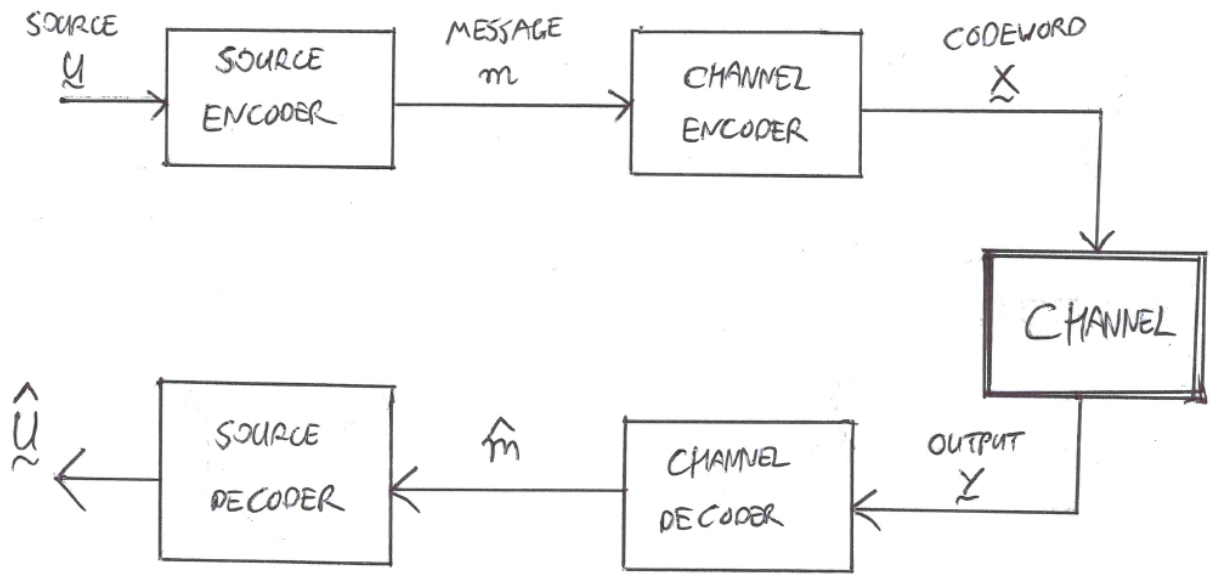
\includegraphics[width=0.95\linewidth]{cs3236-full-communication-setup.png} 

  for input $x$, output $y$, input alphabet $\mathcal{X}$, output alphabet $\mathcal{Y}$

  \begin{itemize}
    \item \definition{channel} medium over which we transmit information
      \begin{itemize}
        \item \definition{discrete} input/output alphabets $\mathcal{X}$ and $\mathcal{Y}$ are finite
        \item \definition{memoryless} outputs are (conditionally) independent: $\mathbb{P}[Y=y \vert X=x] = \Pi^n_{i=1} P_{Y \vert X} (y_i \vert x_i)$
      \end{itemize}
  \end{itemize}

  \begin{minipage}[c]{0.3\linewidth}
    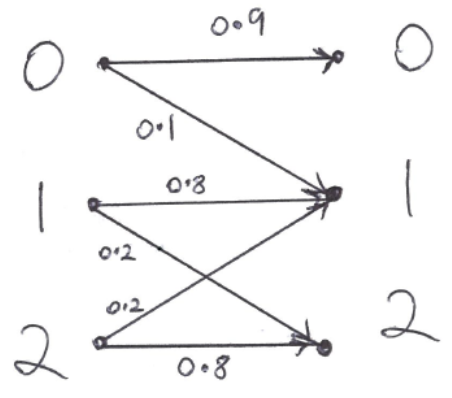
\includegraphics[width=0.95\linewidth]{cs3236-channel-transition-diagram-2.png} 
  \end{minipage}
  \begin{minipage}[c]{0.65\linewidth}{\textcolor{black}{
        \definition{probabilistic modelling approach} when the input is $x \in \mathcal{X}$, a given output $y \in  \mathcal{Y}$ is produced with probability $P_{Y \vert X} (y \vert x)$ 
        \\$\quad$ - see channel transition diagram
    }}
  \end{minipage}

  \begin{itemize}
    \item \definition{error probability} $P_e = \mathbb{P}[\hat{m} \neq m]$
      \begin{itemize}
        \item assuming uniform distribution
        \item on non-uniform distribution: can use  $P_{e_i \text{max}}$
      \end{itemize}
    \item \definition{rate} $R = \frac{1}{n} \log_2 M \quad$ for block length $n$
      \begin{itemize}
        \item higher rate = sending faster (opposite of source coding where lower is better)
        \item = $\frac{k}{n}$ for sending $k$ bits
        \item $R \leq 1$ for binary channels
      \end{itemize}
  \end{itemize}

  \subsection{Channel Capacity}

  \begin{itemize}
    \item \definition[, $C$]{channel capacity} maximum of all rates $R$ such that, for any target error probability $\epsilon > 0$, there exists a block length $n$ and codebook $\mathcal{C} = \{x^{(1)}, \dots, x^{(M)}\}$ with $M=2^{nR}$ codewords such that $P_e \leq \epsilon$
  \end{itemize}

  \begin{tightcenter}
    \ildefinition{channel coding theorem} 

    for any discrete memoryless channel $C(P_{Y \vert X})$,
    we have \( {\displaystyle{ C=\max_{P_x} I(X;Y) }} \) 
  \end{tightcenter}

  \begin{itemize}
    \item \textit{capacity-achieving input distribution}: input distribution $P_X$ that maximises the mutual information
      \begin{itemize}
        \item we can maximise $P_X$, but cannot control $I(X;Y)$
        \item usually (but not always) uniform for "symmetric" channels
      \end{itemize}
    \item (\textbf{achievability}) for any $R<C$, there exists a code of rate $\geq R$ with arbitrarily small $P_e$
    \item (\textbf{converse}) for any $R>C$, any code rate $\geq R$ cannot have arbitrarily small $P_e$ (for any codebook)
    \item examples
      \begin{itemize}
        \item noiseless channel ($\mathcal{X} = \mathcal{Y} = \{0,1\}$) (deterministic): 
          \( {\displaystyle{ C=\max_{P_X} I(X;Y) = \max_{P_X} H(X) = 1 }} \) 
        \item binary symmetric channel ($\mathcal{X} = \mathcal{Y} = \{0,1\}$):
          $P_{Y\vert X}(y \vert x) = \begin{cases} 1-\delta &y=x \\ \delta &y=1-x \end{cases} $
          \( {\displaystyle{ C = \max_{P_X} I(X;Y) = \max_{P_X} (H(Y) - H_2 (\delta)) }} \) 
          \( {\displaystyle{ \,\quad = \max_{P_X} (H_2( \mathbb{P}[Y=1]) - H_2 (\delta)) = 1-H_2(\delta) }} \) 
          \begin{itemize}
            \item we can't maximise $\mathbb{P}[Y=1]$ directly but we can let $P_X$ be uniform to get $P_Y(1) = \frac{1}{2}$
          \end{itemize}
        \item binary erasure channel ($\mathcal{X} = \{0,1\}, \mathcal{Y} = \{0,1,e\}$):
          \begin{minipage}[c]{0.75\linewidth}
            \begin{itemize}
              \item for \textit{erasure probability} $\epsilon$ \\
                $P_{Y \vert X} (y \vert x) = \begin{cases} 1-\epsilon &y=x \\ \epsilon &y=e \\ 0 &y=1-x \end{cases}$
            \end{itemize}
          \end{minipage}
          \begin{minipage}[c]{0.2\linewidth}
            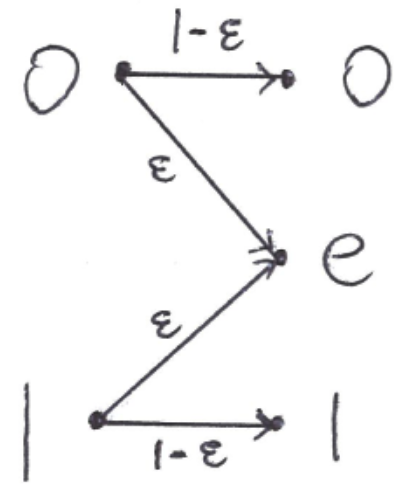
\includegraphics[width=0.95\linewidth]{cs3236-binary-erasure-channel.png} 
          \end{minipage}
          \( {\displaystyle{ C = \max_{P_X} I(X;Y) = \max_{P_X} ( H(X) - H(X\vert Y) ) }} \) 
          \( {\displaystyle{ \,\quad = \max_{P_X} (H(X) - \epsilon H(X)) = 1-\epsilon }} \) 
          \begin{itemize}
            \item maximising $H(Y)$ doesn't work here - you can't get an arbitrary $P(Y)$ distribution
          \end{itemize}
      \end{itemize}
  \end{itemize}

  \subsection{Jointly Typical Sequences}

  \begin{tightcenter}
    a pair of $(\mathbf{x}, \mathbf{y})$ of length-$n$ input and output sequences is \ildefinition{jointly typical}  wrt a joint distribution $P_{XY}$ if 
    $2^{-n(H(X)+\epsilon)} \leq P_X(\mathbf{x}) \leq 2^{-n(H(X)-\epsilon)}$
    $2^{-n(H(Y)+\epsilon)} \leq P_Y(\mathbf{y}) \leq 2^{-n(H(Y)-\epsilon)}$
    $2^{-n(H(X,Y)+\epsilon)} \leq P_{XY}(\mathbf{x}, \mathbf{y}) \leq 2^{-n(H(X,Y)-\epsilon)}$
  \end{tightcenter}

  \begin{itemize}
    \item aka: the $X$ sequence, $Y$ sequence, and joint $(X,Y)$ sequence are all typical
    \item \definition[, $\mathcal{T}_n(\epsilon)$]{jointly typical set} the set of all jointly typical sequences
    \item a joint distribution on sequences: $P_{\mathbf{x}, \mathbf{y}}(\mathbf{x}, \mathbf{y}) = \Pi^n_{i=1} P_{XY} (x_i, y_i)$ - independent product
  \end{itemize}

  \subsubsection{properties}

  \begin{enumerate}
    \item (\textbf{equivalent definition}) $\quad(\mathbf{x}, \mathbf{y}) \in \mathcal{T}_n(\epsilon) \iff $
      $\quad H(X) - \epsilon \leq \frac{1}{n} \sum^n_{i=1} \log_2 \frac{1}{P_X(x_i)} \leq H(X) + \epsilon$
      $\quad H(Y) - \epsilon \leq \frac{1}{n} \sum^n_{i=1} \log_2 \frac{1}{P_Y(y_i)} \leq H(Y) + \epsilon$
      $H(X, Y) - \epsilon \leq \frac{1}{n} {\displaystyle{\sum^n_{i=1}}} \log_2 \frac{1}{P_Y(x_i, y_i)} \leq H(X, Y) + \epsilon$

    \item (\textbf{high probability}) \\*
      $\mathbb{P}[(\mathbf{X}, \mathbf{Y}) \in \mathcal{T}_n(\epsilon)] \to 1$ as $n \to \infty$
      \begin{itemize}
        \item because law of large numbers on the above 3 
      \end{itemize}
    \item (\textbf{cardinality upper bound}) \\*
      \( {\displaystyle{ \vert \mathcal{T}_n(\epsilon) \vert \leq 2^{n(H(X,Y)+\epsilon)} }} \) 
    \item (\textbf{probability for independent sequences}) \\*
      if $(\mathbf{X}', \mathbf{Y}') \sim P_X(\mathbf{x}')P_Y(\mathbf{y}')$ are independent copies of  $(\mathbf{X}, \mathbf{Y})$, then the probability of joint typicality is 
      $\mathbb{P}[(\mathbf{X}', \mathbf{Y}') \in \mathcal{T}_n(\epsilon)] \leq 2^{-n(I(X;Y)-3\epsilon)}$
      \begin{itemize}
        \item intuition: for an independent draw from X and an independent draw from Y (instead of joint distribution), the probability of being typical is much lower
        \item mutual information (computed from joint distribution): how far X,Y are from being independent
      \end{itemize}
  \end{enumerate}

  \subsection{Achievability via Random Coding}

  for codebook $\mathcal{C} = \{ \mathbf{x}^{(1)}, \dots, \mathbf{x}^{(M)} \}$, where $m$ is encoded into length-$n$ sequence $\mathbf{x}^{(m)} = ( x_1^{(m)}, \dots, x_n^{(m)} )$

  \begin{itemize}
    \item idea: prove the existence of a good codebook without explicitly constructing it 
      \begin{itemize}
        \item for some random $\mathcal{C}$, show $\mathbb{E}[P_e(\mathcal{C})] \leq \epsilon$ 
          \\* (thus $\exists$ some $\mathcal{C}$ with $P_e \leq \epsilon$)
        \item let each codeword be i.i.d. according to $P_X$
      \end{itemize}
    \item \definition{random coding} generate each symbol $X_i^{(m)}$ of each codeword randomly and independently according to some distribution $P_X$.
      \begin{itemize}
        \item \textit{encoder}: maps $m$ to $\mathbf{X}^{(m)} = (X_1^{(m)}, \dots, X_n^{(m)})$
        \item \textit{decoder}: form estimate  $\hat{m}$ from output sequence $\mathbf{Y} = (Y_1, \dots, Y_n)$
          \begin{itemize}
            \item if $!\exists m'$ s.t. $(\mathbf{X}^{(m')}, \mathbf{Y}) \in \mathcal{T}_n(\epsilon)$, set $\hat{m} = m'$
              \begin{itemize}
                \item if there is a single index where the codeword and received sequence are jointly typical
              \end{itemize}
            \item else give up (treat as error)
          \end{itemize}
      \end{itemize}
    \item for $\mathbf{X}^{(m)}$ transmitted (i.e. correct $m$)
      \begin{itemize}
        \item $(\mathbf{X}^{(m)}, \mathbf{Y})$ is i.i.d. on $P_{XY} = P_X \times P_{Y \vert X}$
        \item since $P_{\mathbf{Y} | \mathbf{X}}$ is i.i.d. according to $P_{Y \vert X}$, $\mathbf{X}^{(m)}$ is i.i.d. according to $P_X$ (by construction)
      \end{itemize}
    \item for $\mathbf{X}^{(\hat{m})}$ not transmitted (i.e. incorrect $\hat{m}$),
      \begin{itemize}
        \item $(\mathbf{X}^{(m')}, \mathbf{Y}) \sim P_\mathbf{X}(\mathbf{x}')P_\mathbf{Y}(\mathbf{y}')$
        \item joint distribution is an independent product - $\mathbf{Y}$ only depends on $\mathbf{X}^{(m)}$, and $P_{\mathbf{X}}$ is i.i.d.
      \end{itemize}
  \end{itemize}

  \subsubsection{error probability}

  \begin{itemize}
    \item we have $\hat{m} = m$ if:
      \begin{enumerate}
        \item $(\mathbf{X}^{(m)}, \mathbf{Y})$ is jointly typical
        \item none other $(\mathbf{X}^{(\hat{m})}, \mathbf{Y})$ is jointly typical (with $\hat{m} \neq m$)
      \end{enumerate}
    \item $\mathbb{P}[$success$] \geq \mathbb{P}[\textcircled{1}$ and $\textcircled{2}]$ $\Rightarrow$ $\mathbb{P}[$failure$] \leq \mathbb{P}[$not $\textcircled{1} \;\cup$ not $\textcircled{2}]$
  \end{itemize}
  \begin{align*}
    P_e &\leq \mathbb{P}[(\mathbf{X}^{\scriptscriptstyle(m)}, \mathbf{Y}) \not\in \mathcal{T}_n(\epsilon) \cup \bigcup_{\scriptscriptstyle m' \neq m} \{ (\mathbf{X}^{\scriptscriptstyle(m')}, \mathbf{Y}) \in \mathcal{T}_n(\epsilon) \} ] 
     \\ &\leq \mathbb{P}[(\mathbf{X}^{\scriptscriptstyle(m)}, \mathbf{Y}) \not\in \mathcal{T}_n(\epsilon)] + \sum_{\hat{m} \neq m} \mathbb{P}[(\mathbf{X}^{\scriptscriptstyle(\hat{m})}, \mathbf{Y}) \not\in \mathcal{T}_n(\epsilon)]
     \\ &\leq \delta_n + \sum_{\hat{m} \neq m} 2^{-n(I(X;Y) - 3\epsilon)} \text{ where } \delta\to 0 \text{ as } n\to\infty
     \\ &\leq \delta_n + M \times 2^{-n(I(X;Y) - 3\epsilon)} 
  \end{align*}

  \begin{itemize}
    \item $R < I(X;Y) - 3\epsilon$ since $M = 2^{nR}$ $\Rightarrow$ thus $P_e$ can be arbitrarily small for any rate $R$ arbitrarily close to $I(X;Y)$
    \item choose $P_X$ to achieve $C = \max_{P_x} I(X;Y)$
    \item then we can get vanishing error probability rates for rates arbitrarily close to capacity $C$
  \end{itemize}







\end{multicols*}

\end{document}
